\setcounter{equation}{0} \numberwithin{equation}{section}

\section{Thoreau}
You never gain something but that you lose something.\\
		-- Thoreau
\section{Unknown}
And dropping a barbell he points to the sky\\

\begin{figure}[h]
\centering
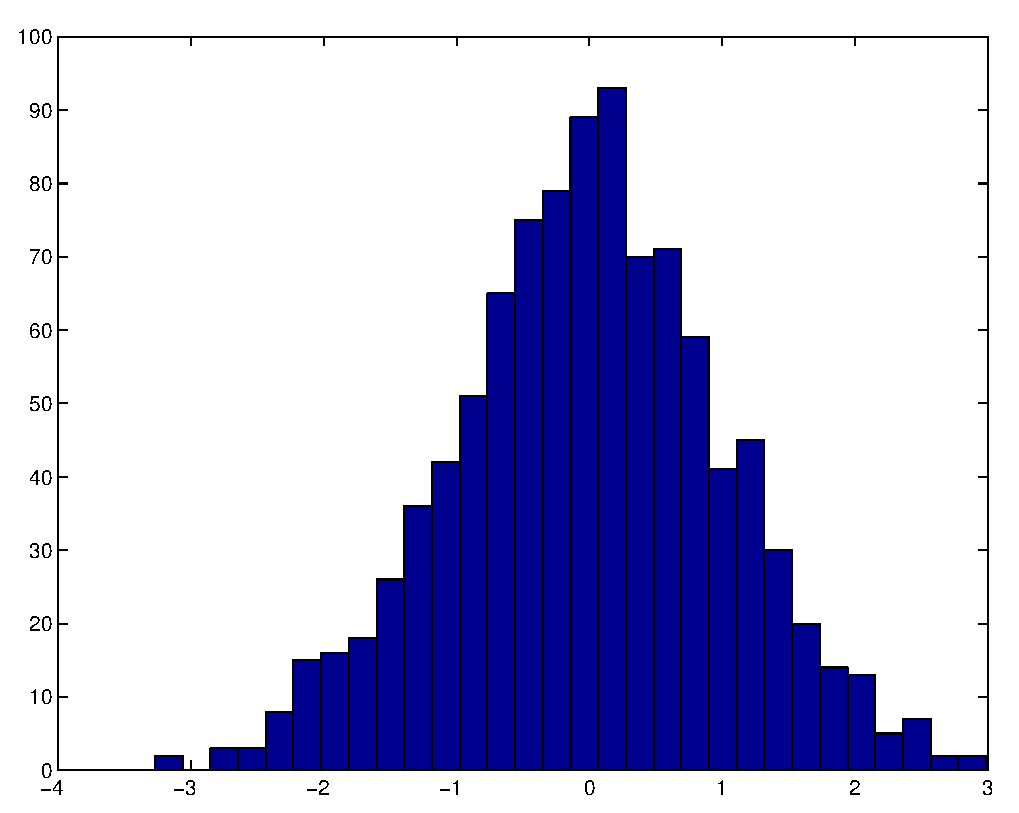
\includegraphics[width = 4.5 in ]{figure.eps}
\caption{Caption of a figure.}\label{FigureLabel}
\end{figure}

\begin{table}[h]
\centering \caption{The values of test
statistics and the corresponding critical values
at~$t_0.$~~$\alpha=0.1.$~}\label{stanford}\vskip .1in
\begin{tabular}{|c|c|c|c|c|c|c|}\hline
$t_0$ & 30 & 60 & 90 & 120 & 150 & 180 \\ \hline
Critical Value & 11.2282 & 10.5357 & 11.1108 & 11.7942 & 11.7343 & 11.7471\\ \hline
Test Statistic & 25.3182 & 24.6395 & 24.6049 & 25.6623 & 27.1320 & 29.3247\\ \hline
\end{tabular}
\end{table}

\section{Citations}

%If you use the package natbib for citations, here is the example how to cite an article.
%Many thanks to Dr. Maria Rizzo who worked this section.

To cite an article use cite, citet, or citep.

For ``in text'' citations use citet:  The original result is attributed to \citet{vn28}.
Refer to \citet{mardia70} for an example.
Refer to \cite{mardia70} for an example.

For a ``parenthetical citation'' use citep:  The computations were implemented in R \citep{R}
using bootstrap \citep{dh97,et93}.

When citing a book, it is helpful to mention where to find the result by indicating
a chapter or a page number or an equation number:  \citet[Ch.~6]{et93} discuss additional results.


%If you don't want to use natbib, you should insert comment (\%) in the above part.  
%Here is the example to cite an article without using natbib package. \cite{forina1991class}
